\section{Modeling uncontrolled intersections}
\label{sec:modeling_uncontrolled}
Each rule is modeled with a first-order formula.
A formula is a combination of atomic formulas,
logical connectives and quantifiers.
We identify some subformulas 
that have an intuitive intended meaning
as \emph{auxiliary predicates}.
This is to simplify the expression of long formulas.

Atomic formulas represent either \emph{events} or \emph{static facts}.
The events and static facts are defined in terms of mathematical concepts,
such as shapes, curves, sets, intersection, union, collision (the first time two sets intersect), etc.
An \emph{event} is represented by a predicate with time as one of the arguments.
A \emph{static fact} is represented by a predicate without time as an argument.

We use Herbrand semantics to interpret the formulas \cite{Herbrand.2019}.
A traffic scenario is described by
a finite collection of ground atomic formulas which
represent static facts and events.
Therefor, traffic rules are grounded on traffic scenarios.
This choice of semantics provides
a more intuitive interpretation (than a Tarskian semantics.)
Furthermore,
implementation becomes straightforward using Answer Set Programming.

In modeling traffic rules,
we avoid using function symbols.
Therefore,
each Herbrand model (of some traffic rules and a traffic scenario) is finite.
For example,
the domain of a quantifier on a time variable $T$ is
the set of all timestamps observed in the traffic scenario.

\subsection{Traffic Rules}
In this section,
we model the logical form of
the traffic rules.
In the fragment of handbook that we analyzed,
we identified three rules:
Rule \ref{rule:yieldToInside},
\ref{rule:FIFO} and \ref{rule:yieldToRight}.
Here we present the formula for each rule
using the predicates that were introduced in the analysis.
%------------------------
\subsubsection{Rule (\ref{rule:yieldToInside})}
\begin{center}
    $ mustYieldToForRule(V1, V2, yieldToInside) \leftrightarrow $ \\
    $ \Big( atTheIntersection(V1) \; \land $\\
    $ inTheIntersection(V2) \Big) $

\end{center}
In our model of the yield obligation,
we keep track of who must yield to whom,
and an identifier for the corresponding rule
(e.g. $yieldToInside$).
The identifier accounts for the fact that
the mapping from the yield obligations to the actions
depends on the rule corresponding to the obligation.
This will become clear in the definition of
$mustStopToYield$.

%------------------------
\subsubsection{Rule (\ref{rule:FIFO})}
\begin{center}
    $ mustYieldToForRule(V2, V1, firstInFirstOut) \leftrightarrow $ \\
    $ \Big( atTheIntersection(V1) \; \land $\\
    $ atTheIntersection(V2) \; \land $\\
    $ arrivedEarlierThan(V1, V2) \Big) $
\end{center}

%------------------------
\subsubsection{Rule (\ref{rule:yieldToRight})}
\begin{center}
    $ mustYieldToForRule(V1, V2, yieldToRight) \leftrightarrow $ \\
    $ \Big( atTheIntersection(V1) \; \land $\\
    $ atTheIntersection(V2) \; \land $\\
    $ arrivedSameTime(V1, V2) \; \land $\\
    $ isOnRightOf(V2, V1) \Big) $
\end{center}

%-------------------------
\subsubsection{The yield action}
In the case of an uncontrolled intersection,
there is no explicit definition of the yield action in the driver handbook.
We interpret the \emph{yield} action to be \emph{stopping and waiting for a certain amount of time}.
The duration of wait depends on the rule corresponding to the yield obligation.
For rules $firstInFirstOut$ and $yieldToRight$,
we define the duration to be 
until the other vehicle enters the intersection;
thus the duration is 
the same as of the yield obligation.
However,
for rule $yieldToInside$,
the duration depends on a notion of lane \emph{reservation}.
The predicate $mustStopToYield$ defines the yield action:
\begin{center}
    $ mustStopToYield(V1) \; \leftrightarrow \; \exists V2 \Bigg( $ \\
    $ \exists L \Big(  mustYieldToForRule(V1, V2, yieldToInside) \; \land $\\
    $ requestedLane(V1, L) \; \land \; reservedLane(V2, L) \Big) $\\
    $ \lor $ \\
    $ mustYieldToForRule(V1, V2, firstInFirstOut) $ \\
    $ \lor $ \\
    $ mustYieldToForRule(V1, V2, yieldToRight) $ \Bigg).
\end{center}

\subsection{Auxiliary Predicates}

%----------------------------------
\subsubsection{At the intersection}
\begin{center}
    $ atTheIntersection(V) \; \leftrightarrow \; \Big(  arrived(V) \; \land \; \neg entered(V) \Big) $
\end{center}
where
\begin{center}
    $ arrived(V) \; \leftrightarrow \; (\exists F)(\exists T) arrivedAtForkAtTime(V, F, T) $
\end{center}
and
\begin{center}
    $ entered(V) \; \leftrightarrow \; (\exists F)(\exists T) enteredForkAtTime(V, F, T) $.
\end{center}
The predicates $arrivedAtForkAtTime$ and $enteredForkAtTime$
represent the events
\emph{arrival at an intersection} and
\emph{entering an intersection}, respectively.
The time parameter $T$ in these predicates
is called a \emph{time stamp}.

%----------------------
\subsubsection{In the intersection}
\begin{center}
    $ inTheIntersection(V) \; \leftrightarrow \; \Big(  entered(V) \; \land \; \neg exited(V) \Big) $
\end{center}
where
\begin{center}
    $ exited(V) \; \leftrightarrow \; (\exists E)(\exists T) exitedFromAtTime(V, E, T) $.
\end{center}

%----------------------
\subsubsection{Arrival precedence}
\begin{center}
    $ arrivedEarlierThan(V1, V2) \; \leftrightarrow $ \\
    $ (\exists T1)(\exists T2) \Big( arrivedAtTime(V1, T1) \; \land $ \\
    $ arrivedAtTime(V2, T2) \; \land \; T1 < T2 \Big).$
\end{center}
where
\begin{center}
    $ arrivedAtTime(V, T) \; \leftrightarrow \; (\exists F) arrivedAtForkAtTime(V, F, T) $.
\end{center}

The $arrivedSameTime$ is similar,
except `$=$' instead of `$<$'.
%----------------------
\subsubsection{On-the-right-of relation for vehicles}
\begin{center}
    $ isOnRightOf(V1, V2) \; \leftrightarrow \; (\exists F1)(\exists F2)(\exists T1)(\exists T2) \Big( $ \\
    $ arrivedAtForkAtTime(V1, F1, T1)\; \land $ \\
    $ arrivedAtForkAtTime(V2, F2, T2) \; \land \; isOnRightOf(F1, F2) \Big).$
\end{center}
The latter $isOnRightOf$ is a static fact between two forks.

%-----------------------------------
\subsubsection{Lane request}
At arriving at an intersection,
a vehicle must communicate (to other vehicles) its path through the intersection.\footnote{In fact, a vehicle must signal starting at 100 feet from the intersection \cite[p. 61]{DMV-California.2019}}
The turn signal is used to communicate that.
We say a vehicle \emph{requests} an intersection-lane using its turn signal.\footnote{Note that
due to the limited communication capacity of a turn signal,
more than one lane may be requested.
For example,
a left-turn signal could mean a U-turn,
or a left-turn to a crossing street.}

An \emph{intersection lane} is a lane
that connects an incoming lane of the intersection to an outgoing lane.
A \emph{fork} is the collection of all intersection lanes from an incoming lane.
Therefore,
an incoming lane uniquely identifies a fork, and vice versa.

Each intersection-lane determines
which turn signal must be used
if a vehicle wants to pass through the intersection using that lane.
That signal is called the \emph{correct signal} for the lane.

Therefore,
a lane $L$ is requested by a vehicle $V$,
if $V$ signaled the correct signal for $L$
when arriving at $L$'s fork $F$:
\begin{center}
    $ requestedLane(V, L) \; \leftrightarrow  $ \\
    $ (\exists S)(\exists F) \Big( signaledAtFork(V, S, F) \; \land $ \\
    $ branchOf(L, F) \; \land \; laneCorrectSignal(L, S) \Big). $
\end{center}
where
\begin{center}
    $ signaledAtFork(V, S, F) \; \leftrightarrow \; (\exists T) signaledAtForkAtTime(V, S, F, T) $
\end{center}
and
\begin{center}
    $ branchOf(L, F) \; \leftrightarrow \; (\exists E) laneFromTo(L, F, E) $.
\end{center}



%-----------------------------------
\subsubsection{Lane reservation}
We say that
a vehicle inside the intersection \emph{reserves} a lane $L$,
to indicate that it started passing through the intersection
and its path (may) pass through (portions of) $L$,
so it is not safe for other vehicles to use $L$.
We assume that the reserving vehicle's path through the intersection
will be consistent with their requested lane(s).\footnote{\label{foot:limitations}See \S \ref{sec:limitations} for more discussion on this.}
A vehicle $V$ \emph{reserves} a lane $L1$ if
\begin{enumerate}
    \item 
    $V$ requested $L1$ and $V$ is on $L1$,
    or if
    \item
    $V$ requested $L2$,
    $V$ is on $L2$,
    the lanes overlap (i.e. intersect),
    and $V$ has not left the overlapping lane $L1$ yet.
\end{enumerate}
Formally:
\begin{center}
    $ reservedLane(V, L1) \; \leftrightarrow $ \\
    $ \Bigg(  \Big(  requestedLane(V, L1) \; \land \; isOnLane(V, L1) \Big) \; \lor $ \\
    $ \exists L2 \Big( requestedLane(V, L2) \; \land \; isOnLane(V, L2) \; \land$ \\
    $ overlaps(L2, L1) \; \land \neg leftTheLane(V, L1) \Big) \Bigg).$
\end{center}
where
\begin{center}
    $ leftTheLane(V, L) \; \leftrightarrow \; (\exists T) leftLaneAtTime(V, L, T) $.
\end{center}
The predicate $leftTheLane(V, L)$ indicates that
vehicle $V$ entered lane $L$ and then left $L$.
For most intersection geometries,
this implies that $V$ will not enter $L$ again.
For example,
observe the pair of intersecting lanes in Figure~\ref{fig:lane-intersection}.
If a vehicle passes the intersection through one of these lanes,
it will enter and leave the other lane only once.\footnotemark[\ref{foot:limitations}]
\begin{figure}
\centering
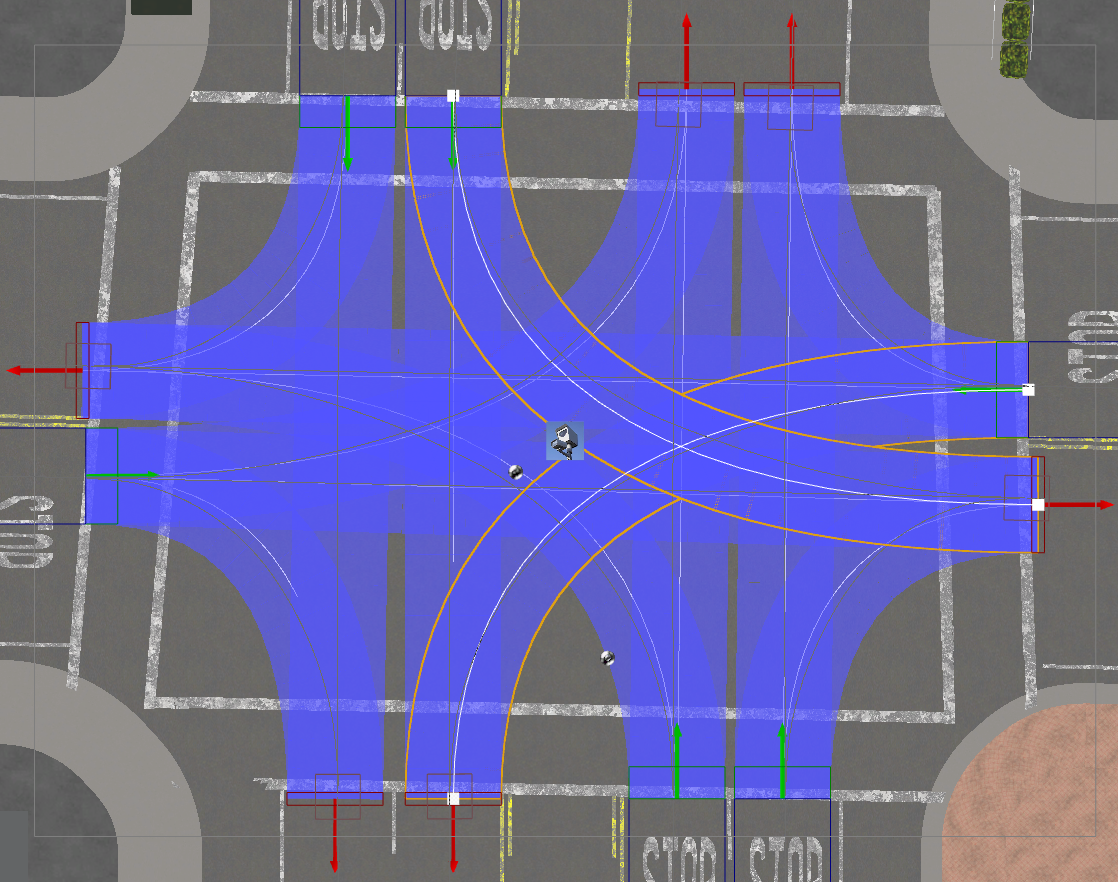
\includegraphics[width=0.5\linewidth]{figures/chapter3/lane_intersection.png}
\caption{Intersecting lanes.}
\label{fig:lane-intersection}
\vspace{-0.5cm}
\end{figure}

\subsection{Events}

%-------------------------------
\subsubsection{Time stamp}
A \emph{time stamp} is a numerical representation of the global clock.
In real time,
one event may strictly precede another but the time difference be imperceptible to humans.
Hence, it is reasonable to assume that
real time events that are closer (in time) than a threshold,
happened at the same time.
Therefore, we adopt a discrete view of time.
That is, a timestamp is simply the number of time steps since the beginning of a scenario.
The length of a time step is a hyperparameter to our model.
%-------------------------------
\subsubsection{Arrival event}
The predicate $arrivedAtForkAtTime(V, F, T)$ represents
the event of vehicle $V$ arriving at the intersection
from fork $F$ at time $T$.
The \emph{arrival time} is when the vehicle intersects with the \emph{arrival box}.
%-------------------------------
\subsubsection{Turn signal event}
The predicate $signaledAtForkAtTime(V, S, F, T)$ represents
the event of vehicle $V$ using turn signal $S$
when it arrives at fork $F$ at time $T$.
%----------------------
\subsubsection{Entrance event}
The predicate $enteredForkAtTime(V, F, T)$ represents
the event of vehicle $V$ entering (branches of) fork $F$ at time $T$.
An \emph{entrance box} represents
the border between the incoming lane and the branches of $F$.
%----------------------
\subsubsection{Lane leave event}
The predicate $leftLaneAtTime(V, L, T)$ represents
the event of vehicle $V$ leaving lane $L$ completely at time $T$.
That is,
at time $T$,
intersection of $V$ and $L$ transitions from nonempty to empty.
%----------------------
\subsubsection{Exit event}
The predicate $ exitedFromAtTime(V, E, T) $ represents the event of
vehicle $V$ leaving the intersection
from the \emph{exit} $E$
at time $T$.
The time $T$ is when the vehicle's body stops intersecting
the exit $E$'s extent box.
The \emph{extent box} is simply a box-shaped subset of the 3D space.


\subsection{Static predicates}
In this section we define
the static predicates identified in the traffic rules.
The arguments of the predicates are traffic-related objects
such as lane, turn signal, etc.

%--------------------------------
\subsubsection{Intersection lane}
An \emph{intersection lane} is a lane
that connects an incoming lane to an outgoing lane
of the intersection.
A \emph{lane} is a tube-shaped volume
that is curved along its length
and has a rectangular cross section.
The \emph{center} of the lane is a spline curve
along the length of the tube.
The left and right boundaries of an intersection lane
are offsets of the center by half of the lane width.
The \emph{width} of a lane changes
from the width of the incoming lane to the width of the outgoing lane.
This change is linear
with respect to the length of the center curve from the incoming lane.
The bottom of the lane aligns on the pavement.
In Figure \ref{fig:intersection-lane}
we see an example of left-turn,
right-turn,
and no-turn intersection lanes.

\begin{figure}% >>>
  \centering
  \begin{minipage}[t]{.43\linewidth}
    {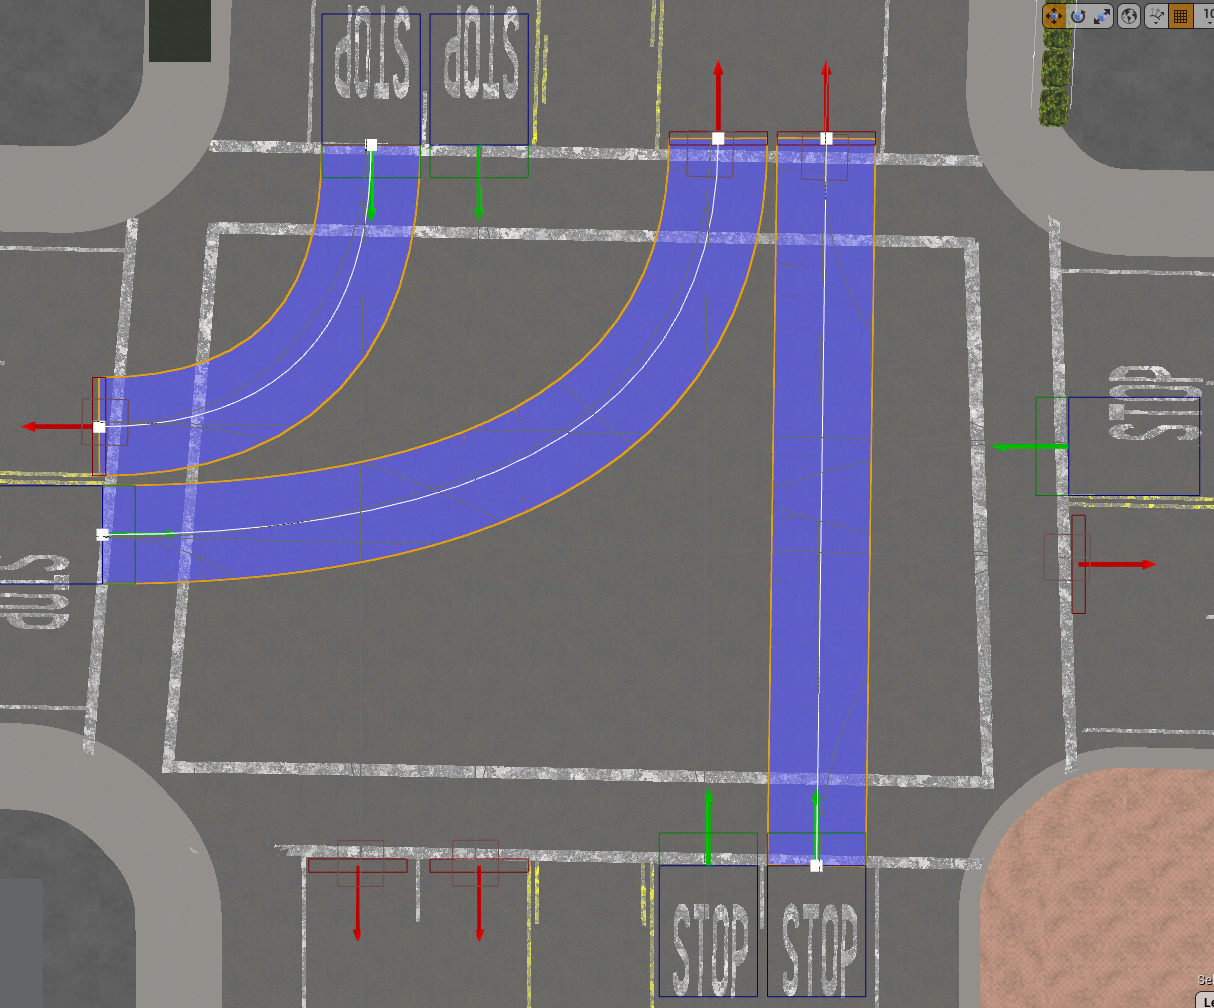
\includegraphics[width=\linewidth]{figures/chapter3/intersection-lane.png}}%
    \subcaption{Top view}
  \end{minipage}%
  \hfill
  \begin{minipage}[t]{.555\linewidth}
    {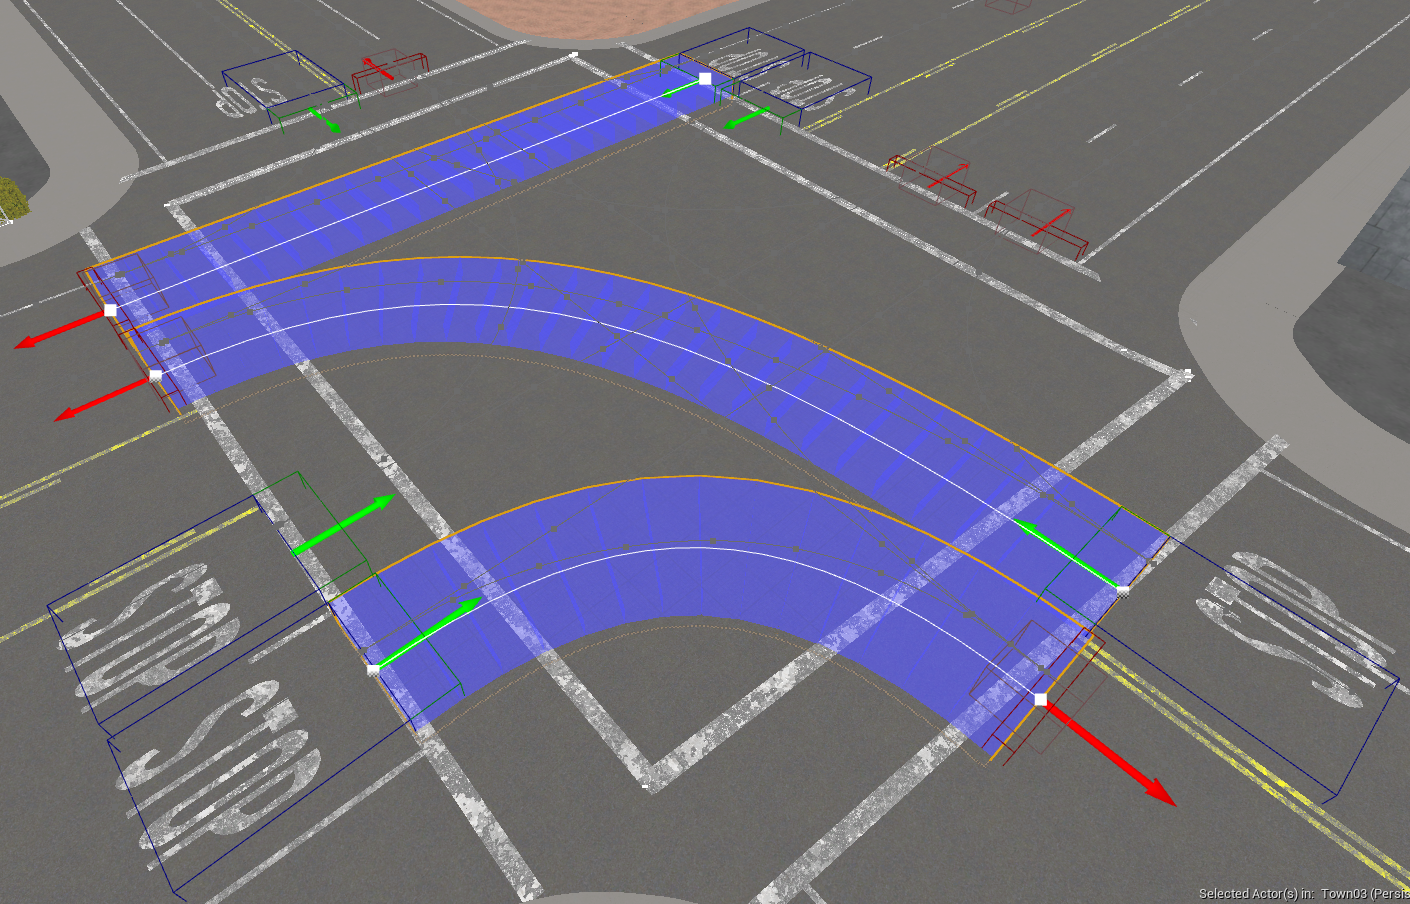
\includegraphics[width=\linewidth]{figures/chapter3/intersection-lane_perspective.png}}%
    \subcaption{Perspective view}
  \end{minipage}%
  \caption{Examples of intersection-lane geometry.}\label{fig:intersection-lane}%
\end{figure}% <<<
%-------------------
\subsubsection{Fork}
A \emph{fork} is the set of
all intersection-lanes that start from the same incoming lane.
Each intersection-lane is called a \emph{branch} of its fork.
Since there is a one-to-one correspondence between forks and incoming lanes,
we can identify a fork with an incoming lane or vice versa.
%--------------------------
\subsubsection{Lane overlaps}
The predicate $overlaps$ holds for a pair of intersection lanes if
their regions intersect.
Therefore, it defines a symmetric relation.
%--------------------------
\subsubsection{Is-on-right-of relation for forks}
We define $isOnRightOf(F2, F1)$ for two forks,
based on their corresponding incoming lanes.
The relation $isOnRightOf$ must be irreflexive and anti-symmetric.\footnote{That is,
no fork is to the right of itself;
and if $F2$ is on the right of $F1$ then
$F1$ is not on the right of $F2$.}
The driver handbook does not give a clear definition.
We define this relation based on angles between vectors.
The direction of an incoming lane
defines a 2D vector on the plane (i.e. the pavement).
We say $F2$ is \emph{on the right of} $F1$ if the angle of $F2$ relative to $F1$,
measured counterclockwise,
is more than 30 and less than 150 degrees.\footnote{The Federal Highway Administration recommends that
``in the design of new facilities or redesign of existing facilities where right-of-way is restricted,
intersecting roadways should meet at an angle of not less than 75 degrees.''\cite{FHWA.2001}
However,
as we see in Figure \ref{fig:on-the-right-of} (c),
the north side of 46th St is 40 degrees to the right of Pico Way.
Therefore,
we choose a conservative infimum of 30 degrees.}
The direction \emph{counterclockwise} is with respect to a downward view of the intersection from above.

For example,
consider Figure \ref{fig:on-the-right-of} (b).\footnote{Intersection of
Harrison Street and Providence Street, Worcester, Massachusetts.}
It shows the incoming lanes
and the angles between consecutive lanes.
Then, as expected intuitively,
the predicate $isOnRightOf$ holds for the following pairs:
$(East, South)$,
$(North, East)$,
$(West, North)$, and
$(South, West)$.
Under our definition,
more than one leg of an intersection may be on the right of another leg.
For example,
consider Figure \ref{fig:on-the-right-of} (c).\footnote{Intersection of
46sth St, F St, and Pico Way, Sacramento, California.}
The F Street and Pico Way are 50 degrees and 140 degrees from south side of 46th Street,
counterclockwise.
Hence, both of them are on the right of (the south side of) 46th Street.
\begin{figure}% >>>
  \centering
  \begin{minipage}[b]{.3\linewidth}
    \subcaptionbox{Definition}
      {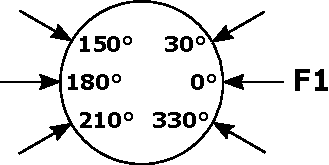
\includegraphics[width=\linewidth]{figures/chapter3/onTheRightOf_Horizontal.pdf}}
    \subcaptionbox{Example.}
      {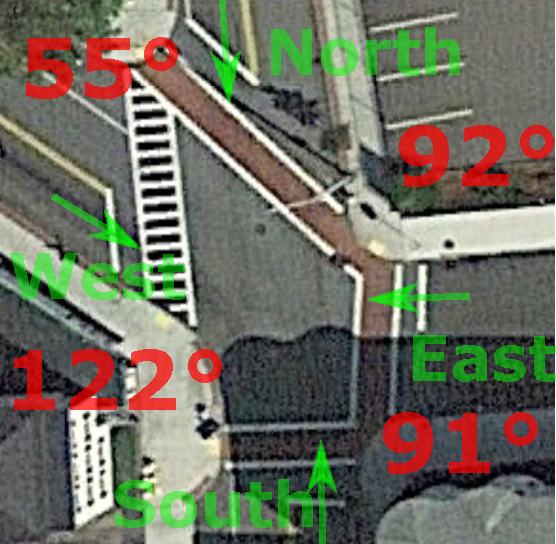
\includegraphics[width=\linewidth]{figures/chapter3/onTheRightOf_Harison-Providence.pdf}}%
  \end{minipage}%
  \hspace*{5mm}
  \begin{minipage}[t]{.3\linewidth}
    \subcaptionbox{Multiplicity}
      {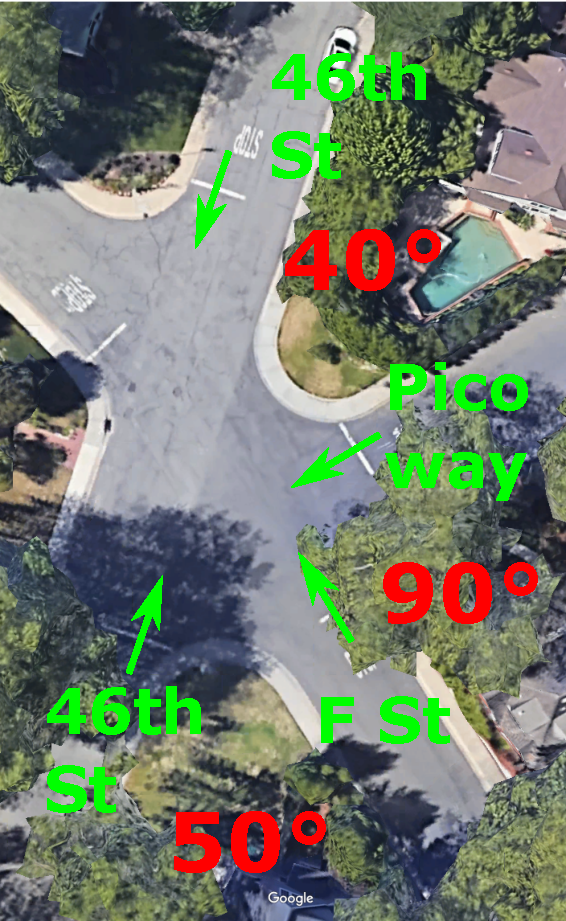
\includegraphics[width=\linewidth]{figures/chapter3/onTheRightOf_F-46th.pdf}}%
  \end{minipage}%
  \caption
  {%
    Is-on-right-of relation for forks.%
    \label{fig:on-the-right-of}%
  }%
\end{figure}% <<<

If the angle from $F1$ to $F2$ is in the interval $[0, 30]$ or $[330, 360)$,
then the incoming lanes are considered heading the same direction,
i.e. on the same street.
If the angle is in $[150, 210]$
we say $F2$ is \emph{in front of} $F1$
i.e. vehicles on $F2$ are \emph{oncoming traffic} relative to $F1$.
If the angle is in $(210, 330)$,
then $F2$ is on the left of $F1$,
i.e. $F1$ is on the right of $F2$.

%--------------------------
\subsubsection{Arrival box}
The \emph{arrival box} is 
a box on an incoming lane that starts at
a pre-specified distance from the intersection (i.e. before the end of the incoming lane)
and ends at the border between the incoming lane and the intersection.
This distance is the \emph{length} of the box.
The \emph{width} of the box is the width of the arriving lane.
The length of the box is a hyperparameter.
For example,
in Figure \ref{fig:arrival-line},
the dark-blue boxes at the crosswalk lines,
designate the boundaries of the arrival box.
In this example,
the length of the box is 4 meters.
When a vehicle overlaps an arrival box,
an arrival event is generated.

\begin{figure}
\centering
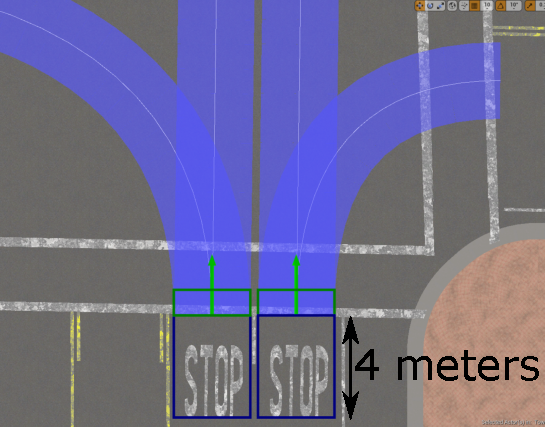
\includegraphics[width=.5\linewidth]{figures/chapter3/arrival-line.pdf}
\caption{Arrival box.}
\label{fig:arrival-line}
\vspace{-0.5cm}
\end{figure}

%--------------------------
\subsubsection{Entrance box}
This box is used to generate the entrance event.
It marks the boundary between an incoming lane and the intersection area.
Each fork has an entrance box.
%--------------------------
\subsubsection{Lane-from-to}
The predicate $laneFromTo(L, F, E)$
indicates that lane $L$ starts at fork $F$ and ends at exit $E$.
Therefore,
this predicate specifies the possible routes through the intersection.

